% JK: I think give an overview here of the experiments here
%     and what you're going to show in this section (and why)
In this section we compare the schedules created by solving the ILP formulation
given in Section~\ref{sec:methods} to schedules that were manually generated,
in terms of adherence to the hard and soft constraints outlined in Section~\ref{sec:problem}.
We also want to analyze the efficiency of the ILP approach in generating schedules
by its runtime on a variety of instances that may be found in the real-world.
Our goal is to show that the schedules provided by solving the ILP successfully
enforce all hard constraints and improve satisfiability of soft constraints, 
as well as to demonstrate that our ILP formulation can be used for a wide range
of configurations.

\subsection{Implementation}
We developed a Python software package with a user interface that implements the above
linear program and allows configuration of clinicians at~\cite{...}, to be
% JK: what is this ref? Do you want to mention it is in Python?
% TODO: I will add a ref to our Github repo here, once I clean it up and open source it
used by the ID division at St.\ Michael's Hospital. The software was used to
generate the results in the following sections, using real data as well as
simulated data as input. All the following experiments were conducted on an
Intel Core i7-4770k CPU @ 3.50 GHz with 16 GB of RAM running 64-bit Windows 10.
Our software package uses COIN-OR Branch-and-Cut open source solver
% JK: "software" here is not clear to me, is it the solver for the ILP formulation?
version 2.9.9~\cite{johnjforrest_coin-or/cbc:_2019}.

\subsection{Comparison with Manually Generated Schedules}  %main comment  = I think use past
%tense in writing
We used clinician time-off requests and minimum/maximum requirements from
2015-2018 as input data for the ILP problem.
Table~\ref{tbl:2018-schedule-comparison} compares the optimal schedule generated using
the software with the manually-created schedule for data from 2018. The
schedule is color-coded to distinguish between the different clinicians.

% Table generated by Excel2LaTeX from sheet '2018'
\begin{table}[h]
%	\tiny
 	\centering
 	\begin{adjustbox}{scale=0.8}
	    \begin{tabular}{c||ccc||ccc}
	    	\multicolumn{1}{c||}{\multirow{2}[1]{*}{Week \#}} & \multicolumn{3}{c||}{LP Solution}                                                                                                                                       & \multicolumn{3}{c}{Historical Data}                                                                                                                                     \\
	    	                                                  &                  HIV                  &                                 ID                                 &                              Weekend                               &                  HIV                  &                                 ID                                 &                              Weekend                               \\ \midrule\midrule
	    	                        1                         & \cellcolor[rgb]{ .663,  .816,  .557}A &                \cellcolor[rgb]{ .957,  .69,  .518}E                &                \cellcolor[rgb]{ .957,  .69,  .518}E                & \cellcolor[rgb]{ .663,  .816,  .557}A &                \cellcolor[rgb]{ .957,  .69,  .518}E                &               \cellcolor[rgb]{ .459,  .443,  .443}H                \\
	    	                        2                         & \cellcolor[rgb]{ .663,  .816,  .557}A &                \cellcolor[rgb]{ .957,  .69,  .518}E                &                \cellcolor[rgb]{ .518,  .592,  .69}G                & \cellcolor[rgb]{ .663,  .816,  .557}A &                \cellcolor[rgb]{ .957,  .69,  .518}E                &               \cellcolor[rgb]{ .663,  .816,  .557}A                \\
	    	                        3                         & \cellcolor[rgb]{ .608,  .761,  .902}B &               \cellcolor[rgb]{ .557,  .663,  .859}F                &               \cellcolor[rgb]{ .557,  .663,  .859}F                & \cellcolor[rgb]{ .608,  .761,  .902}B &               \cellcolor[rgb]{ .459,  .443,  .443}H                &                \cellcolor[rgb]{ .518,  .592,  .69}G                \\
	    	                        4                         & \cellcolor[rgb]{ .608,  .761,  .902}B &               \cellcolor[rgb]{ .557,  .663,  .859}F                &               \cellcolor[rgb]{ .459,  .443,  .443}H                & \cellcolor[rgb]{ .608,  .761,  .902}B &               \cellcolor[rgb]{ .459,  .443,  .443}H                & \cellcolor[rgb]{ .251,  .251,  .251}\textcolor[rgb]{ 1,  1,  1}{I} \\
	    	                        5                         & \cellcolor[rgb]{ .663,  .816,  .557}A &                \cellcolor[rgb]{ .518,  .592,  .69}G                &               \cellcolor[rgb]{ .663,  .816,  .557}A                & \cellcolor[rgb]{ .663,  .816,  .557}A &                \cellcolor[rgb]{ .518,  .592,  .69}G                &               \cellcolor[rgb]{ .557,  .663,  .859}F                \\
	    	                        6                         & \cellcolor[rgb]{ .663,  .816,  .557}A &                \cellcolor[rgb]{ .518,  .592,  .69}G                &                \cellcolor[rgb]{ .957,  .69,  .518}E                & \cellcolor[rgb]{ .663,  .816,  .557}A &                \cellcolor[rgb]{ .518,  .592,  .69}G                &                  \cellcolor[rgb]{ 1,  .851,  .4}C                  \\
	    	                        7                         &   \cellcolor[rgb]{ 1,  .851,  .4}C    &               \cellcolor[rgb]{ .608,  .761,  .902}B                &                  \cellcolor[rgb]{ 1,  .851,  .4}C                  & \cellcolor[rgb]{ .663,  .816,  .557}A &               \cellcolor[rgb]{ .557,  .663,  .859}F                &               \cellcolor[rgb]{ .608,  .761,  .902}B                \\
	    	                        8                         &   \cellcolor[rgb]{ 1,  .851,  .4}C    &               \cellcolor[rgb]{ .608,  .761,  .902}B                &                \cellcolor[rgb]{ .518,  .592,  .69}G                & \cellcolor[rgb]{ .788,  .788,  .788}D &                  \cellcolor[rgb]{ 1,  .851,  .4}C                  &                \cellcolor[rgb]{ .518,  .592,  .69}G                \\
	    	                        9                         & \cellcolor[rgb]{ .788,  .788,  .788}D &               \cellcolor[rgb]{ .459,  .443,  .443}H                &               \cellcolor[rgb]{ .788,  .788,  .788}D                & \cellcolor[rgb]{ .608,  .761,  .902}B &                  \cellcolor[rgb]{ 1,  .851,  .4}C                  &               \cellcolor[rgb]{ .788,  .788,  .788}D                \\
	    	                       10                         & \cellcolor[rgb]{ .788,  .788,  .788}D &               \cellcolor[rgb]{ .459,  .443,  .443}H                &               \cellcolor[rgb]{ .459,  .443,  .443}H                & \cellcolor[rgb]{ .608,  .761,  .902}B &               \cellcolor[rgb]{ .788,  .788,  .788}D                &               \cellcolor[rgb]{ .459,  .443,  .443}H                \\
	    	                       11                         & \cellcolor[rgb]{ .663,  .816,  .557}A & \cellcolor[rgb]{ .251,  .251,  .251}\textcolor[rgb]{ 1,  1,  1}{I} & \cellcolor[rgb]{ .251,  .251,  .251}\textcolor[rgb]{ 1,  1,  1}{I} & \cellcolor[rgb]{ .663,  .816,  .557}A &               \cellcolor[rgb]{ .608,  .761,  .902}B                &               \cellcolor[rgb]{ .557,  .663,  .859}F                \\
	    	                       12                         & \cellcolor[rgb]{ .663,  .816,  .557}A & \cellcolor[rgb]{ .251,  .251,  .251}\textcolor[rgb]{ 1,  1,  1}{I} &               \cellcolor[rgb]{ .608,  .761,  .902}B                & \cellcolor[rgb]{ .663,  .816,  .557}A &               \cellcolor[rgb]{ .608,  .761,  .902}B                &               \cellcolor[rgb]{ .663,  .816,  .557}A                \\
	    	                       13                         & \cellcolor[rgb]{ .608,  .761,  .902}B &               \cellcolor[rgb]{ .557,  .663,  .859}F                &               \cellcolor[rgb]{ .557,  .663,  .859}F                &   \cellcolor[rgb]{ 1,  .851,  .4}C    &               \cellcolor[rgb]{ .459,  .443,  .443}H                &               \cellcolor[rgb]{ .459,  .443,  .443}H                \\
	    	                       14                         & \cellcolor[rgb]{ .608,  .761,  .902}B &               \cellcolor[rgb]{ .557,  .663,  .859}F                &               \cellcolor[rgb]{ .459,  .443,  .443}H                &   \cellcolor[rgb]{ 1,  .851,  .4}C    &               \cellcolor[rgb]{ .459,  .443,  .443}H                & \cellcolor[rgb]{ .251,  .251,  .251}\textcolor[rgb]{ 1,  1,  1}{I} \\
	    	                       15                         &   \cellcolor[rgb]{ 1,  .851,  .4}C    & \cellcolor[rgb]{ .251,  .251,  .251}\textcolor[rgb]{ 1,  1,  1}{I} &                  \cellcolor[rgb]{ 1,  .851,  .4}C                  & \cellcolor[rgb]{ .608,  .761,  .902}B & \cellcolor[rgb]{ .251,  .251,  .251}\textcolor[rgb]{ 1,  1,  1}{I} &                  \cellcolor[rgb]{ 1,  .851,  .4}C                  \\
	    	                       16                         &   \cellcolor[rgb]{ 1,  .851,  .4}C    & \cellcolor[rgb]{ .251,  .251,  .251}\textcolor[rgb]{ 1,  1,  1}{I} &               \cellcolor[rgb]{ .663,  .816,  .557}A                & \cellcolor[rgb]{ .608,  .761,  .902}B & \cellcolor[rgb]{ .251,  .251,  .251}\textcolor[rgb]{ 1,  1,  1}{I} &                \cellcolor[rgb]{ .957,  .69,  .518}E                \\
	    	                       17                         & \cellcolor[rgb]{ .608,  .761,  .902}B &               \cellcolor[rgb]{ .788,  .788,  .788}D                &               \cellcolor[rgb]{ .788,  .788,  .788}D                & \cellcolor[rgb]{ .663,  .816,  .557}A &                \cellcolor[rgb]{ .957,  .69,  .518}E                &               \cellcolor[rgb]{ .788,  .788,  .788}D                \\
	    	                       18                         & \cellcolor[rgb]{ .608,  .761,  .902}B &               \cellcolor[rgb]{ .788,  .788,  .788}D                &               \cellcolor[rgb]{ .557,  .663,  .859}F                & \cellcolor[rgb]{ .663,  .816,  .557}A &                \cellcolor[rgb]{ .957,  .69,  .518}E                &                \cellcolor[rgb]{ .957,  .69,  .518}E                \\
	    	                       19                         & \cellcolor[rgb]{ .663,  .816,  .557}A &               \cellcolor[rgb]{ .459,  .443,  .443}H                &               \cellcolor[rgb]{ .459,  .443,  .443}H                & \cellcolor[rgb]{ .663,  .816,  .557}A &                  \cellcolor[rgb]{ 1,  .851,  .4}C                  &               \cellcolor[rgb]{ .557,  .663,  .859}F                \\
	    	                       20                         & \cellcolor[rgb]{ .663,  .816,  .557}A &               \cellcolor[rgb]{ .459,  .443,  .443}H                & \cellcolor[rgb]{ .251,  .251,  .251}\textcolor[rgb]{ 1,  1,  1}{I} & \cellcolor[rgb]{ .663,  .816,  .557}A &                  \cellcolor[rgb]{ 1,  .851,  .4}C                  &                  \cellcolor[rgb]{ 1,  .851,  .4}C                  \\
	    	                       21                         & \cellcolor[rgb]{ .788,  .788,  .788}D &                  \cellcolor[rgb]{ 1,  .851,  .4}C                  &                  \cellcolor[rgb]{ 1,  .851,  .4}C                  & \cellcolor[rgb]{ .608,  .761,  .902}B &                \cellcolor[rgb]{ .518,  .592,  .69}G                &               \cellcolor[rgb]{ .663,  .816,  .557}A                \\
	    	                       22                         & \cellcolor[rgb]{ .788,  .788,  .788}D &                  \cellcolor[rgb]{ 1,  .851,  .4}C                  &                \cellcolor[rgb]{ .518,  .592,  .69}G                & \cellcolor[rgb]{ .608,  .761,  .902}B &                \cellcolor[rgb]{ .518,  .592,  .69}G                &                  \cellcolor[rgb]{ 1,  .851,  .4}C                  \\
	    	                       23                         & \cellcolor[rgb]{ .608,  .761,  .902}B &                \cellcolor[rgb]{ .957,  .69,  .518}E                &                \cellcolor[rgb]{ .957,  .69,  .518}E                &   \cellcolor[rgb]{ 1,  .851,  .4}C    &               \cellcolor[rgb]{ .557,  .663,  .859}F                &               \cellcolor[rgb]{ .788,  .788,  .788}D                \\
	    	                       24                         & \cellcolor[rgb]{ .608,  .761,  .902}B &                \cellcolor[rgb]{ .957,  .69,  .518}E                &               \cellcolor[rgb]{ .557,  .663,  .859}F                &   \cellcolor[rgb]{ 1,  .851,  .4}C    &               \cellcolor[rgb]{ .557,  .663,  .859}F                &                  \cellcolor[rgb]{ 1,  .851,  .4}C                  \\
	    	                       25                         & \cellcolor[rgb]{ .663,  .816,  .557}A &               \cellcolor[rgb]{ .459,  .443,  .443}H                &               \cellcolor[rgb]{ .663,  .816,  .557}A                &   \cellcolor[rgb]{ 1,  .851,  .4}C    &                  \cellcolor[rgb]{ 1,  .851,  .4}C                  &                \cellcolor[rgb]{ .518,  .592,  .69}G                \\
	    	                       26                         & \cellcolor[rgb]{ .663,  .816,  .557}A &               \cellcolor[rgb]{ .459,  .443,  .443}H                &               \cellcolor[rgb]{ .459,  .443,  .443}H                & \cellcolor[rgb]{ .788,  .788,  .788}D & \cellcolor[rgb]{ .251,  .251,  .251}\textcolor[rgb]{ 1,  1,  1}{I} &               \cellcolor[rgb]{ .788,  .788,  .788}D                \\
	    	                       27                         & \cellcolor[rgb]{ .608,  .761,  .902}B &                  \cellcolor[rgb]{ 1,  .851,  .4}C                  &                  \cellcolor[rgb]{ 1,  .851,  .4}C                  & \cellcolor[rgb]{ .663,  .816,  .557}A &               \cellcolor[rgb]{ .608,  .761,  .902}B                &                \cellcolor[rgb]{ .957,  .69,  .518}E                \\
	    	                       28                         & \cellcolor[rgb]{ .608,  .761,  .902}B &                  \cellcolor[rgb]{ 1,  .851,  .4}C                  &                \cellcolor[rgb]{ .957,  .69,  .518}E                & \cellcolor[rgb]{ .663,  .816,  .557}A &               \cellcolor[rgb]{ .608,  .761,  .902}B                & \cellcolor[rgb]{ .251,  .251,  .251}\textcolor[rgb]{ 1,  1,  1}{I} \\
	    	                       29                         & \cellcolor[rgb]{ .663,  .816,  .557}A &                \cellcolor[rgb]{ .518,  .592,  .69}G                &               \cellcolor[rgb]{ .663,  .816,  .557}A                & \cellcolor[rgb]{ .608,  .761,  .902}B &               \cellcolor[rgb]{ .788,  .788,  .788}D                &               \cellcolor[rgb]{ .788,  .788,  .788}D                \\
	    	                       30                         & \cellcolor[rgb]{ .663,  .816,  .557}A &                \cellcolor[rgb]{ .518,  .592,  .69}G                &               \cellcolor[rgb]{ .608,  .761,  .902}B                & \cellcolor[rgb]{ .608,  .761,  .902}B &               \cellcolor[rgb]{ .788,  .788,  .788}D                &               \cellcolor[rgb]{ .663,  .816,  .557}A                \\
	    	                       31                         &   \cellcolor[rgb]{ 1,  .851,  .4}C    &               \cellcolor[rgb]{ .557,  .663,  .859}F                &                  \cellcolor[rgb]{ 1,  .851,  .4}C                  &   \cellcolor[rgb]{ 1,  .851,  .4}C    &               \cellcolor[rgb]{ .557,  .663,  .859}F                &                \cellcolor[rgb]{ .957,  .69,  .518}E                \\
	    	                       32                         &   \cellcolor[rgb]{ 1,  .851,  .4}C    &               \cellcolor[rgb]{ .557,  .663,  .859}F                &                \cellcolor[rgb]{ .957,  .69,  .518}E                &   \cellcolor[rgb]{ 1,  .851,  .4}C    &               \cellcolor[rgb]{ .557,  .663,  .859}F                &               \cellcolor[rgb]{ .557,  .663,  .859}F                \\
	    	                       33                         & \cellcolor[rgb]{ .608,  .761,  .902}B &               \cellcolor[rgb]{ .788,  .788,  .788}D                &               \cellcolor[rgb]{ .788,  .788,  .788}D                & \cellcolor[rgb]{ .608,  .761,  .902}B &               \cellcolor[rgb]{ .557,  .663,  .859}F                & \cellcolor[rgb]{ .251,  .251,  .251}\textcolor[rgb]{ 1,  1,  1}{I} \\
	    	                       34                         & \cellcolor[rgb]{ .608,  .761,  .902}B &               \cellcolor[rgb]{ .788,  .788,  .788}D                &               \cellcolor[rgb]{ .608,  .761,  .902}B                & \cellcolor[rgb]{ .608,  .761,  .902}B & \cellcolor[rgb]{ .251,  .251,  .251}\textcolor[rgb]{ 1,  1,  1}{I} &                  \cellcolor[rgb]{ 1,  .851,  .4}C                  \\
	    	                       35                         & \cellcolor[rgb]{ .663,  .816,  .557}A & \cellcolor[rgb]{ .251,  .251,  .251}\textcolor[rgb]{ 1,  1,  1}{I} & \cellcolor[rgb]{ .251,  .251,  .251}\textcolor[rgb]{ 1,  1,  1}{I} & \cellcolor[rgb]{ .663,  .816,  .557}A &                \cellcolor[rgb]{ .518,  .592,  .69}G                &                \cellcolor[rgb]{ .518,  .592,  .69}G                \\
	    	                       36                         & \cellcolor[rgb]{ .663,  .816,  .557}A & \cellcolor[rgb]{ .251,  .251,  .251}\textcolor[rgb]{ 1,  1,  1}{I} &                \cellcolor[rgb]{ .518,  .592,  .69}G                & \cellcolor[rgb]{ .663,  .816,  .557}A &                \cellcolor[rgb]{ .518,  .592,  .69}G                & \cellcolor[rgb]{ .251,  .251,  .251}\textcolor[rgb]{ 1,  1,  1}{I} \\
	    	                       37                         & \cellcolor[rgb]{ .788,  .788,  .788}D &                \cellcolor[rgb]{ .518,  .592,  .69}G                &               \cellcolor[rgb]{ .788,  .788,  .788}D                & \cellcolor[rgb]{ .788,  .788,  .788}D &                  \cellcolor[rgb]{ 1,  .851,  .4}C                  &               \cellcolor[rgb]{ .663,  .816,  .557}A                \\
	    	                       38                         & \cellcolor[rgb]{ .788,  .788,  .788}D &                \cellcolor[rgb]{ .518,  .592,  .69}G                &               \cellcolor[rgb]{ .557,  .663,  .859}F                & \cellcolor[rgb]{ .788,  .788,  .788}D &               \cellcolor[rgb]{ .788,  .788,  .788}D                &                \cellcolor[rgb]{ .957,  .69,  .518}E                \\
	    	                       39                         & \cellcolor[rgb]{ .663,  .816,  .557}A &                \cellcolor[rgb]{ .957,  .69,  .518}E                &               \cellcolor[rgb]{ .663,  .816,  .557}A                & \cellcolor[rgb]{ .663,  .816,  .557}A &               \cellcolor[rgb]{ .608,  .761,  .902}B                &               \cellcolor[rgb]{ .788,  .788,  .788}D                \\
	    	                       40                         & \cellcolor[rgb]{ .663,  .816,  .557}A &                \cellcolor[rgb]{ .957,  .69,  .518}E                &               \cellcolor[rgb]{ .608,  .761,  .902}B                & \cellcolor[rgb]{ .608,  .761,  .902}B & \cellcolor[rgb]{ .251,  .251,  .251}\textcolor[rgb]{ 1,  1,  1}{I} & \cellcolor[rgb]{ .251,  .251,  .251}\textcolor[rgb]{ 1,  1,  1}{I} \\
	    	                       41                         & \cellcolor[rgb]{ .608,  .761,  .902}B &                \cellcolor[rgb]{ .518,  .592,  .69}G                &                \cellcolor[rgb]{ .518,  .592,  .69}G                & \cellcolor[rgb]{ .608,  .761,  .902}B & \cellcolor[rgb]{ .251,  .251,  .251}\textcolor[rgb]{ 1,  1,  1}{I} &                \cellcolor[rgb]{ .518,  .592,  .69}G                \\
	    	                       42                         & \cellcolor[rgb]{ .608,  .761,  .902}B &                \cellcolor[rgb]{ .518,  .592,  .69}G                &                \cellcolor[rgb]{ .957,  .69,  .518}E                & \cellcolor[rgb]{ .788,  .788,  .788}D &               \cellcolor[rgb]{ .557,  .663,  .859}F                &               \cellcolor[rgb]{ .557,  .663,  .859}F                \\
	    	                       43                         & \cellcolor[rgb]{ .788,  .788,  .788}D &                  \cellcolor[rgb]{ 1,  .851,  .4}C                  &               \cellcolor[rgb]{ .788,  .788,  .788}D                &   \cellcolor[rgb]{ 1,  .851,  .4}C    &               \cellcolor[rgb]{ .557,  .663,  .859}F                &                  \cellcolor[rgb]{ 1,  .851,  .4}C                  \\
	    	                       44                         & \cellcolor[rgb]{ .788,  .788,  .788}D &                  \cellcolor[rgb]{ 1,  .851,  .4}C                  & \cellcolor[rgb]{ .251,  .251,  .251}\textcolor[rgb]{ 1,  1,  1}{I} & \cellcolor[rgb]{ .788,  .788,  .788}D &                \cellcolor[rgb]{ .957,  .69,  .518}E                & \cellcolor[rgb]{ .251,  .251,  .251}\textcolor[rgb]{ 1,  1,  1}{I} \\
	    	                       45                         & \cellcolor[rgb]{ .663,  .816,  .557}A &               \cellcolor[rgb]{ .557,  .663,  .859}F                &               \cellcolor[rgb]{ .557,  .663,  .859}F                & \cellcolor[rgb]{ .788,  .788,  .788}D &                \cellcolor[rgb]{ .957,  .69,  .518}E                &                \cellcolor[rgb]{ .957,  .69,  .518}E                \\
	    	                       46                         & \cellcolor[rgb]{ .663,  .816,  .557}A &               \cellcolor[rgb]{ .557,  .663,  .859}F                &               \cellcolor[rgb]{ .663,  .816,  .557}A                & \cellcolor[rgb]{ .663,  .816,  .557}A &               \cellcolor[rgb]{ .608,  .761,  .902}B                &               \cellcolor[rgb]{ .663,  .816,  .557}A                \\
	    	                       47                         &   \cellcolor[rgb]{ 1,  .851,  .4}C    &               \cellcolor[rgb]{ .608,  .761,  .902}B                &                  \cellcolor[rgb]{ 1,  .851,  .4}C                  & \cellcolor[rgb]{ .663,  .816,  .557}A &               \cellcolor[rgb]{ .608,  .761,  .902}B                &               \cellcolor[rgb]{ .788,  .788,  .788}D                \\
	    	                       48                         &   \cellcolor[rgb]{ 1,  .851,  .4}C    &               \cellcolor[rgb]{ .608,  .761,  .902}B                & \cellcolor[rgb]{ .251,  .251,  .251}\textcolor[rgb]{ 1,  1,  1}{I} & \cellcolor[rgb]{ .663,  .816,  .557}A &               \cellcolor[rgb]{ .788,  .788,  .788}D                &                \cellcolor[rgb]{ .518,  .592,  .69}G                \\
	    	                       49                         & \cellcolor[rgb]{ .663,  .816,  .557}A &               \cellcolor[rgb]{ .788,  .788,  .788}D                &               \cellcolor[rgb]{ .788,  .788,  .788}D                & \cellcolor[rgb]{ .663,  .816,  .557}A &               \cellcolor[rgb]{ .788,  .788,  .788}D                &               \cellcolor[rgb]{ .557,  .663,  .859}F                \\
	    	                       50                         & \cellcolor[rgb]{ .663,  .816,  .557}A &               \cellcolor[rgb]{ .788,  .788,  .788}D                &               \cellcolor[rgb]{ .608,  .761,  .902}B                & \cellcolor[rgb]{ .608,  .761,  .902}B &                \cellcolor[rgb]{ .518,  .592,  .69}G                &                \cellcolor[rgb]{ .518,  .592,  .69}G                \\
	    	                       51                         & \cellcolor[rgb]{ .608,  .761,  .902}B &                \cellcolor[rgb]{ .518,  .592,  .69}G                &                \cellcolor[rgb]{ .518,  .592,  .69}G                & \cellcolor[rgb]{ .608,  .761,  .902}B &                \cellcolor[rgb]{ .518,  .592,  .69}G                &                \cellcolor[rgb]{ .957,  .69,  .518}E
	    \end{tabular}%
	\end{adjustbox}
	\caption{Comparison of schedules for 2018}
	\label{tbl:2018-schedule-comparison}%
\end{table}%

% JK: I think use input not include here to avoid unnecessary page breaks
%     https://tex.stackexchange.com/questions/246

First, we evaluated the ILP solution by comparing it with the
% JK: I think it would be good to give a short name for manual and the proposed
%     data -- e.g. LP Solution as in Table 4 and Manual Generation.
%     Then check for consistency throughout.
%     While lack of synonyms can sound repetitive, it can help avoid confusion.
manual generation, as in Table~\ref{tbl:2018-schedule-comparison}. Specifically, we examined the adherence of each
schedule to the constraints presented in Table~\ref{tbl:constraint-summary}. As
shown in Table~\ref{tbl:constraints-comparison}, the ILP solution satisfied all 
hard constraints. In contrast,
% JK: "mandatory" = "hard"? if possible just use one.
manual generation did not satisfy all hard constraints. In
particular, we see that the manual generation assigned clinicians to multiple
consecutive blocks in all four years. Moreover, the manual generation did not have
an equal distribution of weekends and holidays for all four years of data.
Considering all objectives, we see that the ILP solution outperforms manual generation
in all four years, by accommodating almost all time-off requests and
ensuring that weekends are always assigned close to blocks.

% Table generated by Excel2LaTeX from sheet 'constraints'
\begin{table}[h]
	\centering
    \begin{tabular}{l|cc|cc|cc|cc}
    	\hline
    	\multicolumn{1}{c|}{\multirow{2}[1]{*}{\textbf{Constraint}}} & \multicolumn{2}{c|}{\textbf{2015}} & \multicolumn{2}{c|}{\textbf{2016}} & \multicolumn{2}{c|}{\textbf{2017}} & \multicolumn{2}{c}{\textbf{2018}} \\
    	                                                    & LP &      Historical      & LP &      Historical      & LP &      Historical      & LP &     Historical      \\ \midrule
    	Block Coverage                                      & \checkmark  &                      & \checkmark  &                      & \checkmark  &          \checkmark           & \checkmark  &          \checkmark          \\
    	Weekend Coverage                                    & \checkmark  &                      & \checkmark  &                      & \checkmark  &          \checkmark           & \checkmark  &          \checkmark          \\
    	Min/Max                                             & \checkmark  &                      & \checkmark  &                      & \checkmark  &          \checkmark           & \checkmark  &          \checkmark          \\
    	No Consecutive Blocks                               & \checkmark  &                      & \checkmark  &                      & \checkmark  &                      & \checkmark  &                     \\
    	No Consecutive Weekends                             & \checkmark  &                      & \checkmark  &                      & \checkmark  &          \checkmark           & \checkmark  &          \checkmark          \\
    	Equal Weekends                                      & \checkmark  &                      & \checkmark  &                      & \checkmark  &                      & \checkmark  &                     \\
    	Equal Holidays                                      & \checkmark  &                      & \checkmark  &                      & \checkmark  &                      & \checkmark  &                     \\
    	\hline
    	Block Requests                                      &    &                      &    &                      &    &                      &    &                     \\
    	Weekend Requests                                    &    &                      &    &                      &    &                      &    &                     \\
    	Block-Weekend Adjacency                             &    &                      &    &                      &    &                      &    &
    \end{tabular}%
	\caption{Comparison of constraint satisfaction in LP and Historical schedules}
	\label{tbl:constraints-comparison}%
\end{table}%

% JK: If you want to be funny, you can estimate the approximate time to
%     generate the schedule and include that too (16 hours vs 1 second)...

\subsection{Influence of Problem Complexity on Runtime}
Next, we examined the influence of the following four parameters on the
runtime of the ILP solver using simulated data:
number of clinicians;
number of services offered;
number of time-off requests per clinician per year;
time-horizon of the schedule.

% JK: Introduce what you did first and then the figure showing results (see above)
The effect of increasing the number of clinicians and number of services %divisions %do you mean
%services?
on the runtime of the program is shown in Table~\ref{tbl:runtime-services-clinicians-comparison}.
We executed the algorithm for
$S = \{1, 2, 3\}$ total services and $C = \{10, 20, 30, 50\}$ clinicians in
total across all services. 
In a department providing a single service, increasing the number of clinicians
did not affect the runtime, and we were able to find an ILP solution in all four cases
within 1 second.
For 2 concurrent services, a roster of 30 or more
clinicians becomes impractical to schedule, as searching for a solution required
over 24 hours. We saw similar issues for a roster of 20 or more clinicians
assigned to a division with 3 concurrent services. However, when removing the
NCB constraint, we saw a great improvement in runtime for divisions with 2 and 3
services, and we were able to generate a schedule with upwards of 50 clinicians
in under 1.5 seconds.  %what does division mean? do you mean services?

\begin{table}[h]
	\centering
	\begin{tabular}{|c|c||c|c||c|c|}
		\hline
		                                      &  \multicolumn{5}{c|}{Number of Services}  \\ \hline
		\makecell[l]{Number of \\ Clinicians} &  1   &    2    & 2 (CBA) &  3   & 3 (CBA) \\ \hline
		                 10                   & 0.16 &  0.74   &  0.16   & 1.40 &  0.23   \\ \hline
		                 20                   & 0.25 & 7468.86 &  0.32   &  -   &  0.43   \\ \hline
		                 30                   & 0.42 &    -    &  0.49   &  -   &  0.66   \\ \hline
		                 50                   & 0.62 &    -    &  0.82   &  -   &  1.14   \\ \hline
	\end{tabular}
	\caption{Comparison of program runtime (in seconds) for different number of services and total clinicians in the division. `-' indicates that a solution was not found after 24 hours. `CBA' indicates that \underline{c}onsecutive \underline{b}locks were \underline{a}llowed when generating these schedules.}
	\label{tbl:runtime-services-clinicians-comparison}%
\end{table}

% JK: Good to introduce the detault parameters first, then for each parameter explored,
%     Describe what varied.
For the remaining experiments, we simulated a department with 10 clinicians offering 
two services, similar to the department at St.\ Michael's Hospital. 
Each clinician was
configured with $\{0, 5, 10, 15\}$ non-overlapping block
% JK: \abs{BR} does not clearly imply number of blocks (could be confused with week indices),
%     so just leave out the LHS here I think.
% JK: What do you mean by non-overlapping? And why only increments of 5?
requests.
The effect of an increasing number of requests per clinician on the runtime of
the ILP solver is shown in Figure~\ref{fig:runtime-requests}.
The increase in the number of requests did not affect the runtime of
the ILP solver, indicating that it can accommodate a lot of flexibility in
clinician requests. Moreover, we see that all four runs were completed in under
1 second.
% JK: See somments below about trends and repeating simulations.

\begin{figure}[h]
	\centering
	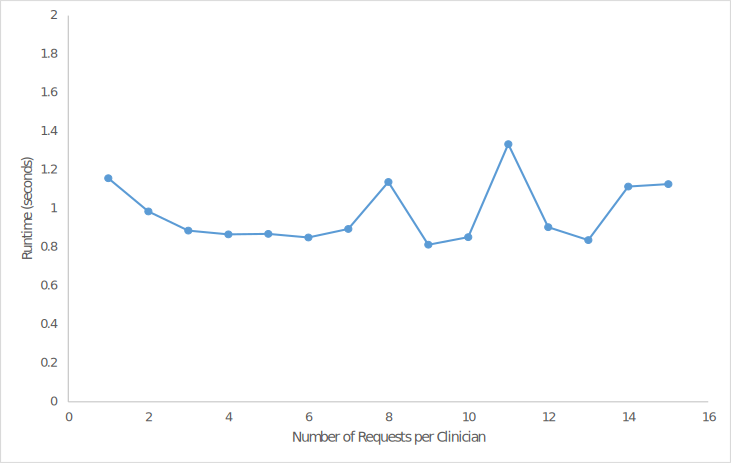
\includegraphics[scale=.5]{fig/runtime_requests} % JK: can you export this to PDF or SVG to avoid pixelation?
	\caption{Runtime of ILP solver with an increasing number of requests per clinician}
  \label{fig:runtime-requests}
  % JK: The trend here is a bit confusing, since I think you're trying to say
  %     that the runtime is not affected by the number of constraints,
  %     but there is noise in these results.
  %     I would re-run this 10-100 times and average the results so that (I expect)
  %     the mean trend is actually flat. You could (should) then also present the runtimes
  %     as box-plots to show that the trend is less than the variability.
\end{figure}

% JK: Introduce what you did first and then the figure showing results (see above)
% JK: Try to introduce these results in the same order as they appear in the
%     first paragraph of this section.
Figure~\ref{fig:runtime-blocks} presents the change in runtime when increasing
the number of 2-week blocks $B = \{26, 52, 78, 104\}$ in a department with 10
clinicians offering two services. There does not seem to be a strong effect on
runtime when we lengthen the time-horizon of the schedule, and in fact the
solver was able to find an optimal schedule for all time horizons within 3
seconds. % 'very reasonable amount of time" is vague. what is reasonable?
%better to give a range in value.
% JK: same comment as above re. trends

\begin{figure}[h]
	\centering
	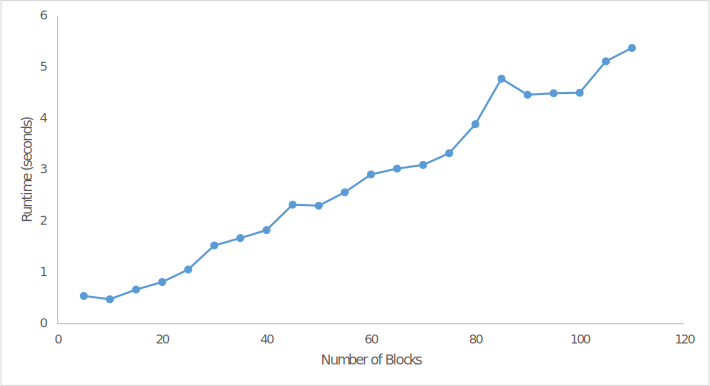
\includegraphics[scale=.5]{fig/runtime_blocks}
	\caption{Runtime of ILP solver with an increasing number of 2-week blocks}%
  \label{fig:runtime-blocks}
  % JK: same comment as above re. trends
  % JK: Thess figures could also possible be Figure 1. a) and b) 
\end{figure}